\documentclass[aspectratio=169]{beamer}
\usetheme{Madrid}
\usepackage{booktabs}
\usepackage{amsmath,amssymb}
\usepackage{tikz}
\usetikzlibrary{arrows.meta,positioning}
\usepackage{pgfplots}
\pgfplotsset{compat=1.18}
\setbeameroption{show notes}

\title[beamer2slides]{beamer2slides}
\subtitle{From a compiled beamer PDF to an editable Google Slides deck}
\author[Demo]{A Demo Author}
\institute[Somewhere]{Somewhere University}
\date{September 2026}

\begin{document}

\begin{frame}
  \titlepage
\end{frame}

\begin{frame}{Outline}
  \tableofcontents
\end{frame}

\section{Why}

\begin{frame}{The problem}
  \begin{itemize}
    \item Slides written in \LaTeX{} are hard to edit together
    \item Google Slides is easy to share and comment on
      \begin{itemize}
        \item but it has no math typesetting
        \item and retyping a talk takes hours
      \end{itemize}
    \item We keep the PDF's layout and make everything editable
  \end{itemize}
  \vspace{1em}
  Inline math stays text where it can: for $x \in \mathbb{R}$ and $n \geq 2$, the mean
  $\bar{x} = \frac{1}{n}\sum_{i=1}^{n} x_i$ is still searchable.
\end{frame}
\note{Mention that the input is the compiled PDF, not the source.}

\section{How}

\begin{frame}{Pipeline}
  \centering
  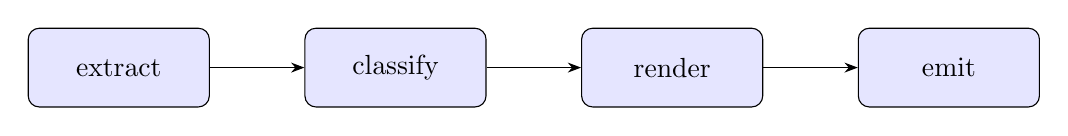
\begin{tikzpicture}[node distance=1.2cm, box/.style={draw, rounded corners, fill=blue!10, minimum width=2.3cm, minimum height=1cm}]
    \node[box] (extract) {extract};
    \node[box, right=of extract] (classify) {classify};
    \node[box, right=of classify] (render) {render};
    \node[box, right=of render] (emit) {emit};
    \draw[-Stealth] (extract) -- (classify);
    \draw[-Stealth] (classify) -- (render);
    \draw[-Stealth] (render) -- (emit);
  \end{tikzpicture}
  \vspace{1.5em}
  \begin{block}{Native where it is faithful}
    Text, lists, tables, blocks and simple diagrams become Slides elements.
  \end{block}
  \begin{alertblock}{Pictures where it is not}
    Display math and complex figures become pictures you can still move.
  \end{alertblock}
\end{frame}

\begin{frame}{Results on the test decks}
  \begin{columns}[T]
    \begin{column}{0.48\textwidth}
      \begin{tabular}{lrr}
        \toprule
        Deck & Slides & Native text \\
        \midrule
        Basic & 4 & 100\% \\
        Math & 3 & 71\% \\
        Figures & 3 & 88\% \\
        Themes & 9 & 94\% \\
        \bottomrule
      \end{tabular}
    \end{column}
    \begin{column}{0.48\textwidth}
      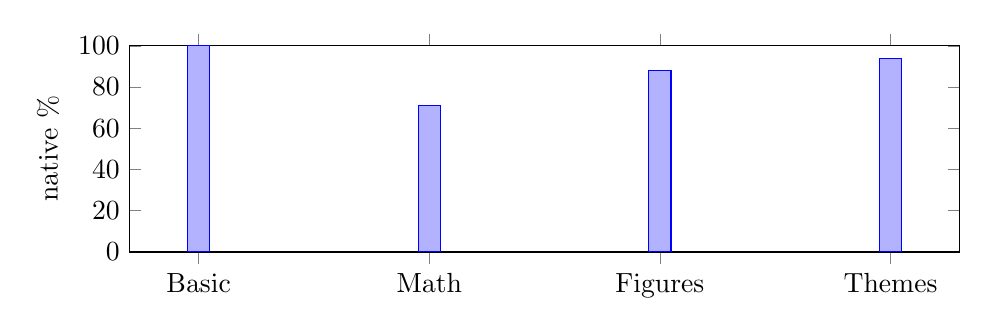
\begin{tikzpicture}
        \begin{axis}[width=\linewidth, height=4.2cm, ybar=0pt, bar width=8pt,
                     symbolic x coords={Basic,Math,Figures,Themes}, xtick=data,
                     ymin=0, ymax=100, ylabel={native \%}]
          \addplot coordinates {(Basic,100) (Math,71) (Figures,88) (Themes,94)};
        \end{axis}
      \end{tikzpicture}
    \end{column}
  \end{columns}
\end{frame}

\begin{frame}{Display math stays exact}
  The least-squares loss
  \begin{equation}
    \mathcal{L}(\theta) = \frac{1}{2n} \sum_{i=1}^{n} \bigl(y_i - f_\theta(x_i)\bigr)^2
  \end{equation}
  is minimised by gradient descent with step size $\eta > 0$:
  \[
    \theta_{t+1} = \theta_t - \eta \, \nabla_\theta \mathcal{L}(\theta_t).
  \]
  \begin{exampleblock}{Try it}
    Move the equation picture: nothing stays behind in the background.
  \end{exampleblock}
\end{frame}
\note{The equations are pictures grouped with nothing; the text around them is editable.}

\section{Try it}

\begin{frame}[fragile]{Usage}
  \begin{enumerate}
    \item Compile your talk as usual
    \item Run the converter on the PDF:
  \end{enumerate}
  \begin{verbatim}
python -m beamer2slides convert talk.pdf
  \end{verbatim}
  \begin{enumerate}
    \setcounter{enumi}{2}
    \item Open the printed link and keep editing in Slides
  \end{enumerate}
\end{frame}

\end{document}
